\section{Approximation Algorithms}

\begin{frame}
  \frametitle{Why should we look for an approximation?}
  \begin{block}{Static graphs}
    \begin{itemize}
      \item many interesting networks are \emph{web-scale};
      \item computing the exact centralities can be extremely expensive;
      \item is there a real reason (i.e., application) to \emph{require} the
        exact values?
    \end{itemize}
  \end{block}
  \pause
  \begin{block}{Dynamic graphs}
    \begin{itemize}
      \item exact centralities change at all times;
      \item not worth chasing for highly volatile quantities;
    \end{itemize}
  \end{block}
  \pause
  In both cases, \emph{high quality} approximations are \emph{sufficient in
  practice}
\end{frame}

\begin{frame}
  \frametitle{What kind of approximation}
  \begin{itemize}
    \item $v$: vertex with exact centrality $c(v)$
    \item $\tilde{c}(v)$: value that ``approximates'' $c(v)$
  \end{itemize}
  \begin{definition}[Absolute error]
    \centering
    $\mathsf{err}_\mathrm{abs}(v)=|c(v)-\tilde{c}(v)|$
  \end{definition}
  \begin{definition}[Relative error]
    \centering
    $\mathsf{err}_\mathrm{rel}(v)=|c(v)-\tilde{c}(v)|/c(v)$
  \end{definition}
  \pause
  \begin{definition}[$(\varepsilon,\delta)$-approximation]
    \begin{itemize}
      \item Let $\varepsilon\in(0,1)$ and $\delta\in(0,1)$;
      \item a \emph{$(\varepsilon,\delta)$-approximation} is a \emph{set}
        $\{\tilde{c}(v), v\in V\}$ of $n$ values, such that
        \[
          \Pr\left(\exists v\in V \text{ s.t. } \mathsf{err}(v)
          >\varepsilon\right)\le \delta;
        \]
        \vspace{-20pt}
      \pause
      \item it offers \emph{uniform probabilistic guarantees} over all the
        nodes;
        \pause
      \item it assumes \emph{normalized} versions of centrality (i.e., in
        $[0,1]$).
    \end{itemize}
  \end{definition}
\end{frame}

\begin{frame}
  \frametitle{Sampling}
  Many of the algorithms we present are \emph{sampling-based}.
  \begin{block}{General Sampling Based Algorithm}
    \begin{enumerate}
      \item Select \emph{independently at random} (not all \emph{uniformly})
        a \emph{small} set of \emph{objects} (e.g., single vertices, pair of vertices, shortest
        paths);
        \pause
      \item Perform some computation using these objects (e.g., SSSP from vertex);
        \pause
      \item Use the results of the computation to estimate the centrality of all
        nodes;
    \end{enumerate}
  \end{block}
\end{frame}

\begin{frame}
  \frametitle{Sampling}
  \begin{block}{Why sampling?}
    By only select a small subset of the ``objects'' (instead of the whole set),
    computing the approximation is faster than computing the exact values
  \end{block}
  \pause
  \begin{block}{Questions for sampling algorithms}
    \begin{itemize}
      \item What ``objects'' to sample?
        \pause
      \item How to sample? If sampling procedure is slow, then the advantages
        are lost;
        \pause
      \item How many objects to sample in order to guarantee an
        $(\varepsilon,\delta)$-approximation?
    \end{itemize}
  \end{block}
\end{frame}

\begin{frame}
  \frametitle{Outline}
  \begin{itemize}
    \item Approximation algorithms for static graphs
      \begin{itemize}
        \item A sampling-based algorithm for closeness
        \item A sampling+pivoting algorithm for closeness
        \item Two sampling-based algorithms for betweenness
      \end{itemize}
    \item Approximation algorithms for dynamic graphs
      \begin{itemize}
        \item Two sampling-based algorithms for betweenness
      \end{itemize}
  \end{itemize}
\end{frame}

\subsection{Approximation Algorithms for Static Graphs}

\begin{frame}
  \centering
  \vfill
  {\huge Fast approximation of centrality}
  \vfill
  {\Large D.~Eppstein, J.~Wang}
  \vfill
  {\large Journal of Graph Algorithms and Applications (2004)}
  \vfill
\end{frame}

\begin{frame}
  \frametitle{Idea}
  \vfill
  Interested in approximating \emph{closeness}:
  \[
    \closeness(x)=\frac{n-1}{\sum_{y\neq x}d(x,y)}
  \]
  (inverse of the average distance)
  \vfill
  Fastest-known exact algorithm: APSP\\
  \qquad I.e., run Dijkstra's algorithm from \emph{each} vertex $v$
  \pause
  \vfill
  Idea: only run Dijkstra from \emph{a few sources}!
  \vfill
  \pause
  \begin{block}{Warning}
    The algorithm actually computes an approximation for
    the \emph{inverse} of closeness:
    \[
      \closeness^{-1}(v)=\frac{\sum_{y\neq x}d(u,v)}{n-1}
    \]
    (effectively the average distance)
  \end{block}
\end{frame}

\begin{frame}
  \frametitle{Algorithm}
  \begin{block}{}
    \begin{itemize}
      \item Let $k$ be the number of sources to obtain the desired
        approximation;
        \pause
      \item For $i=1,\dotsc, k$:
        \begin{itemize}
          \item pick a vertex $u_i$ uniformly at random
            \pause
          \item run Dijkstra from $u_i$
        \end{itemize}
      \item Let
        \[
          \widetilde{\closeness^{-1}}(v)=\frac{n}{n-1}\frac{\sum_{i=1}^k
          d(u_i,v_i)}{k}
        \]
    \end{itemize}
  \end{block}
  \pause
  \begin{theorem}
    $\mathbb{E}\left[\widetilde{\closeness^{-1}}(v)\right]=\closeness^{-1}(v)$.
  \end{theorem}
  \pause
  \begin{block}{Question}
    How large should $k$ be to get a good approximation of $\closeness^{-1}$?
  \end{block}
\end{frame}

\begin{frame}
  \frametitle{Hoeffding Inequality}
  \begin{itemize}
    \item A concentration inequality for the sum of independent random
      variables;
    \item It allows to study the trade-off between the error (difference between
      sample value and expectation) and the sample size;
  \end{itemize}
  \pause
  \begin{theorem}[Hoeffding Inequality]
    Let $x_1,\dotsc, x_n$ be independent r.v., with
    \begin{itemize}
      \item $a_i\le x_i\le b_i$
      \item $\mu=\mathbb{E}[\sum x_i/k]$
    \end{itemize}
    Then, for $\xi > 0$,
    \[
      \Pr\left(\left|\frac{\sum_{i=1}^kx_i}{k}-\mu\right|\ge\xi\right)\le
      2e^{-2k^2\xi^2/\sum_{i=1}^k(b_i-a_i)^2}
    \]
  \end{theorem}
\end{frame}

\begin{frame}
  \frametitle{How much to sample}
  \begin{lemma}
    Let $\Delta$ be the diameter of the graph and let
    $\varepsilon,\delta\in(0,1)$. If
    \[
      k=\Theta\left(\frac{\log n}{\varepsilon^2}\right),
    \]
    Then, \emph{with high probability} (i.e., with probability $\ge 1/n$)
    \[
      \left|\widetilde{\closeness^{-1}}(v)-\closeness^{-1}(v)\right|\le\Delta\varepsilon,
      \text{ for all } v\in V
    \]
  \end{lemma}
  \pause
  Algorithm running time: $O\left(\frac{\log n}{\varepsilon^2}(n\log n +
  m)\right)$.
\end{frame}

\begin{frame}
  \centering
  \vfill
  {\huge Computing Classic Closeness Centrality, at Scale}
  \vfill
  {\Large E.~Cohen, D.~Delling, T.~Pajor, R.~F.~Werneck}
  \vfill
  {\large COSN '14: ACM Conference on Social Networks (2014) }
  \vfill
\end{frame}

\begin{frame}
  \frametitle{Issues with sampling}
  \begin{itemize}
    \item Assume that the distance distribution from a node $v$ has a
      \emph{heavy tail};
    \item the average distance
      \[
        \closeness^{-1}(v)=\frac{\sum_{u\neq v}d(u,v)}{n-1}\enspace
      \]
      is dominated by few distant nodes;
    \pause
    \item it is unlikely that these nodes are among the ones that are sampled
    \pause
    \item Hence the sample average
      \[
        \widetilde{\closeness^{-1}}(v)=\frac{n-1}{n}\frac{\sum_{i=1}d(u_i,v)}{k}
      \]
      is a \emph{poor estimator} of the average distance $\closeness^{-1}(v)$.
  \end{itemize}
\end{frame}

\begin{frame}
  \frametitle{Pivoting}
\end{frame}

\begin{frame}
  \frametitle{Hybrid Estimator}
\end{frame}

\begin{frame}
  \frametitle{Guarantees}
\end{frame}

\begin{frame}
  \frametitle{Experiments}
\end{frame}


\begin{frame}
  \centering
  \vfill
  {\Huge Centrality Estimation in Large Networks}
  \vfill
  {\Large U.~Brandes, C.~Pich}
  \vfill
  {\large International Journal of Bifurcation and Chaos (2007)}
  \vfill
\end{frame}

\begin{frame}
  \frametitle{What kind of approximation do we want?}
  We want uniform quality guarantees on the approximations of all vertices
  \vfill
  Definition:\\
  \quad For $\varepsilon,\delta\in(0,1)$, an $(\varepsilon,\delta)$-approximation is
  a collection $\{\tilde{\betw}(v), v\in V\}$ such that
  \[
    \Pr(\exists v\in V ~:~ |\tilde{\betw}(v) -\betw(v)|>\varepsilon)<\delta
  \]
  $\varepsilon$ controls the accuracy, $\delta$ controls the confidence
  \vfill
  Trade-off: smaller $\varepsilon$ or $\delta$ $\Rightarrow$ higher number of
  samples $\Rightarrow$ slower runtime
\end{frame}

\begin{frame}
  \frametitle{How can one get an $(\varepsilon,\delta)$-approximation?}
  [Brandes and Pich, 2008]: only run SSSP and aggregation from a few sources
  \vfill
  \begin{algorithm}[H]
    \DontPrintSemicolon
    $r\leftarrow \frac{1}{\varepsilon^2}\left(\ln n + \ln 2 +
    \ln\frac{1}{\delta}\right)$ \texttt{// sample size}\;
    $\tilde{\betw}(v)\leftarrow 0$, for all $v\in V$\;
    \For(\texttt{// the exact algorithm would iterate over $V$}){$i\leftarrow 1,\dotsc,r$} {
      $v_i \leftarrow$ random vertex from $V$, chosen uniformly\;
      Perform single-source SP computation from $v_i$\;
      Perform partial aggregation, updating $\tilde{\betw}(u)$, $u\in V$,
      like in exact algorithm\;
    }
    Output $\{\tilde{\betw{v}}, v\in V\}$\;
  \end{algorithm}
  \vfill
  Theorem: The output is an $(\varepsilon,\delta)$-approximation
\end{frame}

\begin{frame}
  \frametitle{How do they prove it?}
  Start with bounding the deviation for a single vertex $v$ (Hoeffding bound):
  \[
    \Pr(|\tilde{\betw}(v)-\betw(v)|>\varepsilon)\le 2e^{-2r\varepsilon^2}
  \]
  \vfill
  Then take the union bound over $n$ vertices to ensure uniform converge\\
  \quad the sample size $r$ must be such that
  \[
    2e^{-2r\varepsilon^2}\le\frac{\delta}{n}
  \]
  That is, to get an $(\varepsilon,\delta)$-approximation, we need
  \[
    r\ge\frac{1}{2\varepsilon^2}\left(\ln n + \ln 2 +
    \ln\frac{1}{\delta}\right)
  \]
\end{frame}

\begin{frame}
  \centering
  \vfill
  {\huge Better Approximation of Betweenness Centrality}
  \vfill
  {\Large R.~Geisberger, P.~Sanders, D.~Schultes}
  \vfill
  {\large ALENEX (2008)}
  \vfill
\end{frame}

\begin{frame}
  \frametitle{Issue with standard estimator}
\end{frame}

\begin{frame}
  \frametitle{New estimator}
\end{frame}

\begin{frame}
  \frametitle{Reduced variance}
\end{frame}

\begin{frame}
  \frametitle{Experiments}
\end{frame}

\begin{frame}
  \centering
  \vfill
  {\huge Fast Approximation of Betweenness Centrality through Sampling}
  \vfill
  {\Large M.~Riondato, E.~M.~Kornaropoulos}
  \vfill
  {\large DMKD: Data Mining and Knowledge Discovery (2015)}
  \vfill
\end{frame}

%\begin{frame}
%  \frametitle{What vertices in a graph are important?}
%  Betweenness centrality is one measure of vertex importance\\
%  \quad Roughly, it is the fraction of Shortest Paths (SP) in a graph that go through a vertex
%  \vfill
%  Let $G=(V,E)$, $|V|=n$, $|E|=m$. The betweenness centrality of $v\in V$ is:
%  \[
%    \betw(v)=\underbrace{\frac{1}{n(n-1)}}_{\mbox{normalization}}\sum_{p_{uw}\in\mathbb{S}_G}
%    \underbrace{\frac{\mathds{1}_{\mathcal{T}_v}(p_{uw})}{\sigma_{uw}}}_{\in [0,1]}
%  \]
%  where:
%  \begin{itemize*}
%    \item $\mathbb{S}_G$: set of all SPs in $G$
%    \item $\mathcal{S}_{uw}$: set of all SPs from $u$ to $w$
%      ($\mathcal{S}_{uw}\subseteq\mathbb{S}_G$,
%      $|\mathcal{S}_{uw}|=\sigma_{uw}$)
%    \item $\mathcal{T}_v$: $\{p\in\mathbb{S}_G ~:~ v\in\mathsf{Int}(p)\}$
%  \end{itemize*}
%\end{frame}
%
%\begin{frame}
%  \frametitle{How to compute betweenness centrality?}
%  Na\"ive algorithm: All Pairs SP computation, followed by aggregation\\
%  \quad Aggregation dominates runtime, $\Theta(n^3)$
%  \vfill
%  [Brandes 2001]: Perform aggregation after each Single-Source SP (SSSP) computation\\
%  \quad Runtime: $O(nm)$ (unweighted $G$), $O(nm + n^2\log n)$ (weighted
%  $G$)\\
%  This is is still too much for graphs with $n=10^9$, $m=10^10$
%  \vfill
%  Possible solution: perform fewer SPs computations by sampling\\
%  \quad We get approximate results, but that's OK!
%  \vfill
%  What kind of approximation do we want ? What should we sample and how much?
%\end{frame}

\begin{frame}
  \frametitle{What is wrong with this approach?}
  1) We need
  \[
    r\ge\frac{1}{2\varepsilon^2}\left(\ln n + \ln 2 +
    \ln\frac{1}{\delta}\right)
  \]
  \begin{itemize}
    \item This is loose, due to the union bound and does not scale well (experiments)
    \item The sample size depends on $\ln n$. This is not the right
      quantity: not all graphs of $n$ nodes are equally ``difficult'': e.g., the $n$-star is ``easier'' than a random graph
  \end{itemize}
  The sample size $r$ should depend on a more-specific characteristic of the graph
  \vfill
  2) At each iteration, the algorithm performs a SSSP computation\\
  \quad Full exploration of the graph, no locality
\end{frame}

\begin{frame}
  \frametitle{How can we improve the sample size?}
  [R. and Kornaropoulos, 2014] present an algorithm that:
  \vfill
  1) uses a sample size which depends on the vertex-diameter, a characteristic
  quantity of the graph. The derivation uses VC-dimension
  \vfill
  2) samples SPs according to a specific, non-uniform distribution over
  $\mathbb{S}_G$. For each sample, it performs a single $s-t$ SP computation
  \begin{itemize}
    \item More locality: fewer edges touched than single-source SP
    \item Can use bidirectional search / A\textsuperscript{*},
      \ldots
  \end{itemize}
\end{frame}

\begin{frame}
  \frametitle{What is the algorithm?}
  \begin{algorithm}[H]
    \DontPrintSemicolon
    $\mathsf{VD}(G)\leftarrow$ vertex-diameter of $G$ \texttt{// stay
    tuned!}\;
    $r\leftarrow\frac{1}{2\varepsilon^2}\left(\lfloor\log_2(\mathsf{VD}(G)-2\rfloor)
    +1 + \ln(1/\delta)\right)$ \texttt{// sample size}\;
    $\tilde{\betw}(v)\leftarrow 0$, for all $v\in V$\;
    \For{$i\leftarrow 1\dotsc,r$}{
      $(u,v)\leftarrow$ random pair of different vertices, chosen
      uniformly\;
      $\mathcal{S}_{uv}\leftarrow$ all SPs from $u$ to $v$ \texttt{//
      Dijkstra, trunc.~BFS, \ldots}\;
      $p\leftarrow$ random element of $\mathcal{S}_{uv}$, chosen
      uniformly \texttt{// not uniform over $\mathbb{S}_G$}\;
      $\tilde{\betw}(w)\leftarrow \tilde{\betw}(w) + 1/r$, for all
      $w\in\mathsf{Int}(p)$ \texttt{// update only nodes along $p$}\;
    }
    Output $\{\tilde{\betw}(v), v\in V\}$
  \end{algorithm}
  Theorem: The output $\{\tilde{\betw}(v), v\in V\}$ is an
  $(\varepsilon,\delta$)-approximation
\end{frame}

\begin{frame}
  \frametitle{VC-dimension}
\end{frame}

\begin{frame}
  \frametitle{How can we prove the correctness?}
  We want to prove that the output $\{\tilde{\betw}(v), v\in V\}$ is an
  $(\varepsilon,\delta$)-approximation
  \vfill
  Let's apply the recipe!

  \begin{enumerate}
    \item  Define betweenness centrality computation as a expectation
      estimation problem (domain $\domain$, family $\family$, distribution
      $\prob$)
    \item Show that the algorithm efficiently samples according to $\prob$
    \item Show how to efficiently compute an upper bound to the VC-dimension\\
      \quad Bonus: show tightness of bound
    \item Apply the VC-dimension sampling theorem
  \end{enumerate}
\end{frame}

\begin{frame}
  \frametitle{How to define the expectation estimation task?}
  \begin{itemize}
    \item The domain $\domain$ is $\mathbb{S}_G$ (all SPs in $G$)\\
    \item The family is $\family=\{\mathds{1}_{\mathcal{T}_v}, v\in V\}$,
      where $\mathcal{T}_v=\{p\in\mathbb{S}_G ~:~: v\in\mathsf{Int}(p)\}$
    \item The probability distribution $\prob$ on $\domain$ is
      \[
        \pi(p_{uw})=\frac{1}{n(n-1)}\frac{1}{\sigma_{uw}}
      \]
      The algorithm samples paths according to $\pi$
  \end{itemize}
  \vfill
  We have
  \[
    \expectation_\pi[\mathds{1}_{\mathcal{T}_v}]=\sum_{p_{uw}\in\mathbb{S}_G}\mathds{1}_{\mathcal{T}_v}\pi(p_{uw})=\sum_{p_{uw}\in\mathbb{S}_G}\mathds{1}_{\mathcal{T}_v}(p_{uw})\frac{1}{n(n-1)}\frac{1}{\sigma_{uw}}=\betw(v)
  \]
\end{frame}

\begin{frame}
  \frametitle{How do we bound the VC-dimension?}
  Definition: The vertex-diameter $\mathsf{VD}(G)$ of $G$ is the maximum
  number of vertices in a SP of $G$
  \[
    \mathsf{VD}(G)=\max\{|p|, p\in\mathbb{S}_G\}
  \]
  If $G$ is unweighted, $\mathsf{VD}(G)=\Delta(G)+1$. Otherwise no relationship\\
  Very small in social networks, even huge ones (shrinking diameter effect)
  \vfill
  Computing $\mathsf{VD}(G)$: $\left(2\frac{\mbox{max.~edge weight}}{\mbox{min.~edge
  weight}}\right)$-approximation via single-source SP
  \vfill
  Theorem: The VC-dimension of $(\mathbb{S}_G,F)$ is at most $\lfloor\log_2\mathsf{VD}(G)
  -2\rfloor +1$
\end{frame}

\begin{frame}
  \frametitle{Let's prove it!}
  Theorem: The VC-dimension is at most $\lfloor\log_2\mathsf{VD}(G)
  -2\rfloor +1$
  \vfill
  Proof:
  \begin{itemize}
    \item For a set $A\subseteq\mathbb{S}_G$ of size $|A|=d$ to be
      shattered, any $p$ in $A$ must appear in at least $2^{d-1}$
      different sets $\mathcal{T}_v$, one for each subset of $A$
      containing $p$.
    \item Any $p$ appears only in the sets $\mathcal{T}_v$ such that
      $v\in\mathsf{Int}(p)$\\
      \quad There are $|\mathsf{Int}(p)|$ such sets
    \item From the definition of the vertex-diameter $\mathsf{VD}(G)$, we have
      $|\mathsf{Int}(p)|\le\mathsf{VD}(G)-2$
    \item To shatter $A$, $d$ must be such that $2^{d-1}\le\mathsf{VD}(G)-2$
    \item So $d$ can be at most $\lfloor\log_2\mathsf{VD}(G) -2\rfloor +1$,
      otherwise $A$ can not be shattered
  \end{itemize}
\end{frame}

\begin{frame}
  \frametitle{How to use the bound?}
  We have that:
  \begin{itemize}
    \item The estimation $\tilde{\betw}(v)$ computed by the algorithm is the
      empirical average for $\betw(v)$
    \item The algorithm samples SPs efficiently according to $\prob$
    \item We know an upper bound to the VC-dimension and how to compute it
      efficiently
  \end{itemize}
  Thus we can apply the VC $\varepsilon$-sample theorem, and obtain that the algorithm
  outputs an $(\varepsilon,\delta)$-approximation:
  \[
    \Pr(\exists v\in V ~:~ |\tilde{\betw}(v)-\betw(v)|>\varepsilon)<\delta
  \]
\end{frame}

\begin{frame}
  \frametitle{Is the bound to the VC-dimension tight?}
  Yes! There is a class of graphs with VC-dimension exactly
  $\lfloor\log_2\mathsf{VD}(G) -2\rfloor +1$\\
  \quad The Concertina Graph Class $(G_i)_{i\in\mathbb{N}}$:
  \begin{figure}[H]
    \centering
    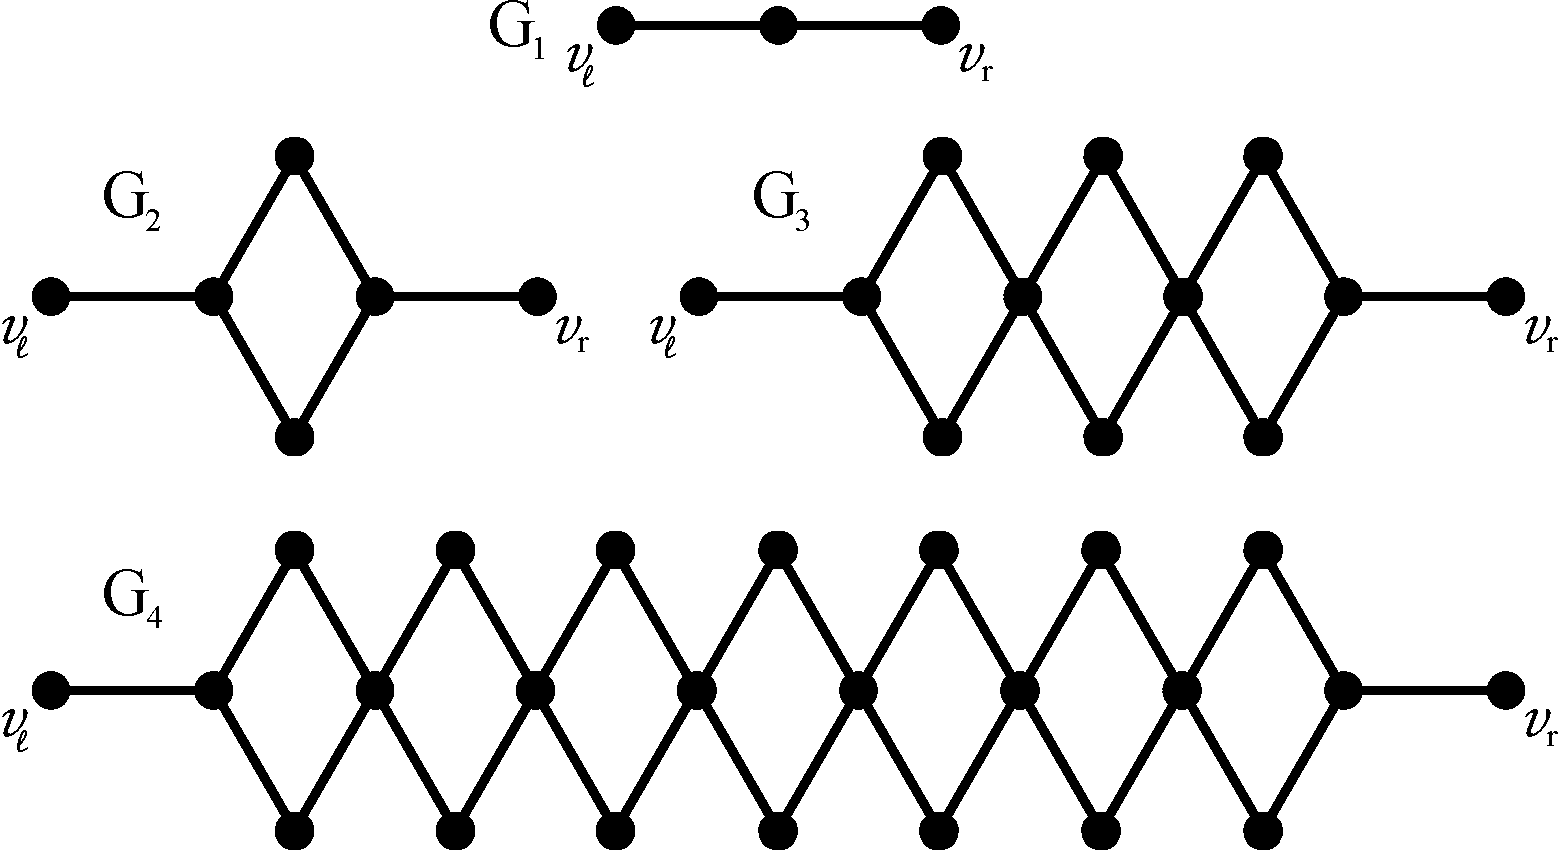
\includegraphics[scale=0.3]{imgs/concertina.pdf}
  \end{figure}
  \vfill
  Theorem: The VC-dimension of $(\mathbb{S}_{G_i}, F)$ is
  $\lfloor\log_2\mathsf{VD}(G) -2\rfloor +1=i$
  \vfill
  Proof Intuition: The middle vertices are internal to a lot of SPs
\end{frame}

\begin{frame}
  \frametitle{Is the Vertex-Diameter the right quantity?}
  No! If $G$ undirected and for every connected pair of nodes there is a
  unique SP, then the VC-dimension is at most 3\\
  \quad These graphs are not just trees!
  \vfill
  Proof: in such a graph, two SPs that meet and separate can not meet again\\
  \quad (+ multiple case analysis)
  \vfill
  The bound ``3'' is tight. In the following graph we can shatter 3 paths
  \begin{figure}[H]
    \centering
    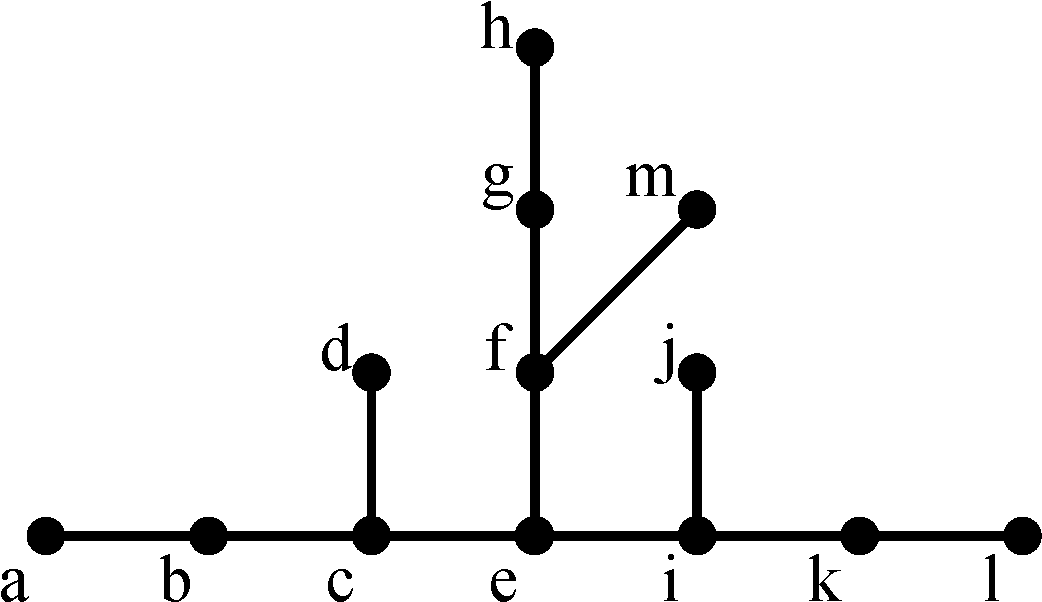
\includegraphics[scale=0.3]{imgs/uniqueshortestpathtight.pdf}
  \end{figure}
  \vfill
  There is room for improvement using pseudodimension (we are working on that!)
\end{frame}

\begin{frame}
  \frametitle{What about directed graphs?}
  Does a similar result also hold for directed graphs with unique SP?\\
  \quad  Not for the same constant $3$. We built a graph with unique SPs between
  all connected nodes and we can shatter a set of $4$ SPs
  \begin{figure}[H]
    \centering
    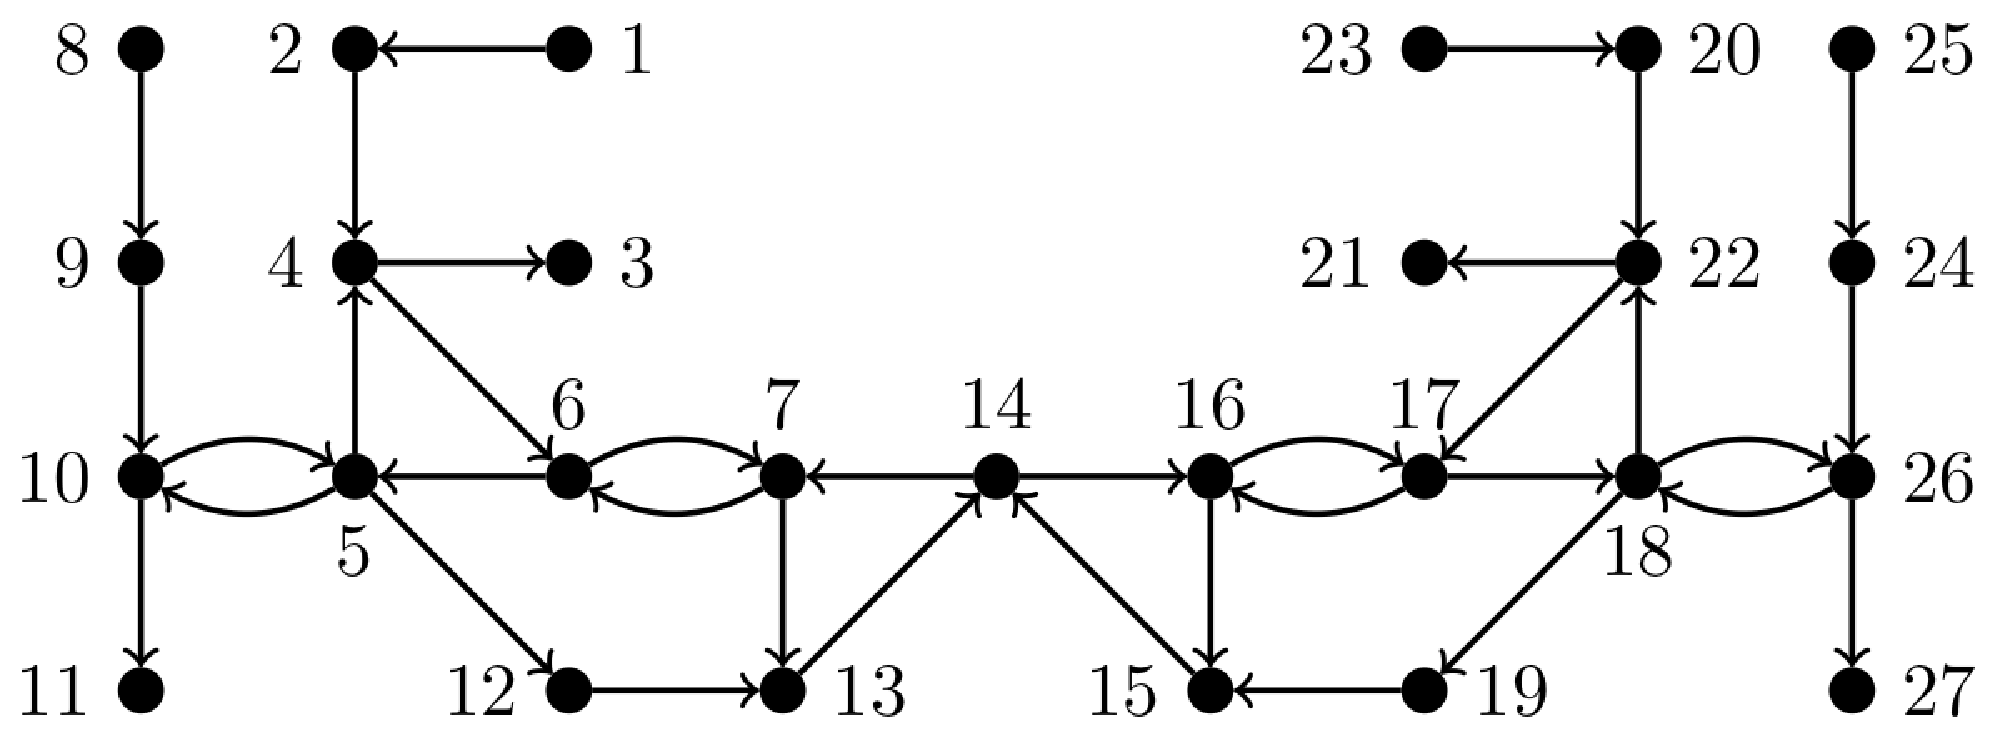
\includegraphics[scale=0.3]{imgs/uniquedirected.pdf}
  \end{figure}
  Yes, finding counterexamples is messy\ldots
  \vfill
  Does it hold for a different constant?\\
  \quad We do not know! Maybe you can work on that?
\end{frame}

\begin{frame}
  \frametitle{How well does the algorithm perform in practice?}
  It performs very well!
  \vfill
  We tested the algorithm on real graphs (SNAP) and on artificial
  Barabasi-Albert graphs, to evalue its accuracy, speed, and scalability
  \vfill
  Results: It blows away the exact algorithm and the union-bound-based
  sampling algorithm
\end{frame}

\begin{frame}
  \frametitle{How accurate is the algorithm?}
  In $O(10^3)$ runs of the algorithm on different graphs and with different
  parameters, we always had $|\tilde{\betw}(v)-\betw(v)|<\varepsilon$ for all
  nodes\\
  \quad Actually, on average $|\tilde{\betw}(v)-\betw(v)|<\varepsilon/8$
  \vfill
  \begin{figure}[H]
    \centering
    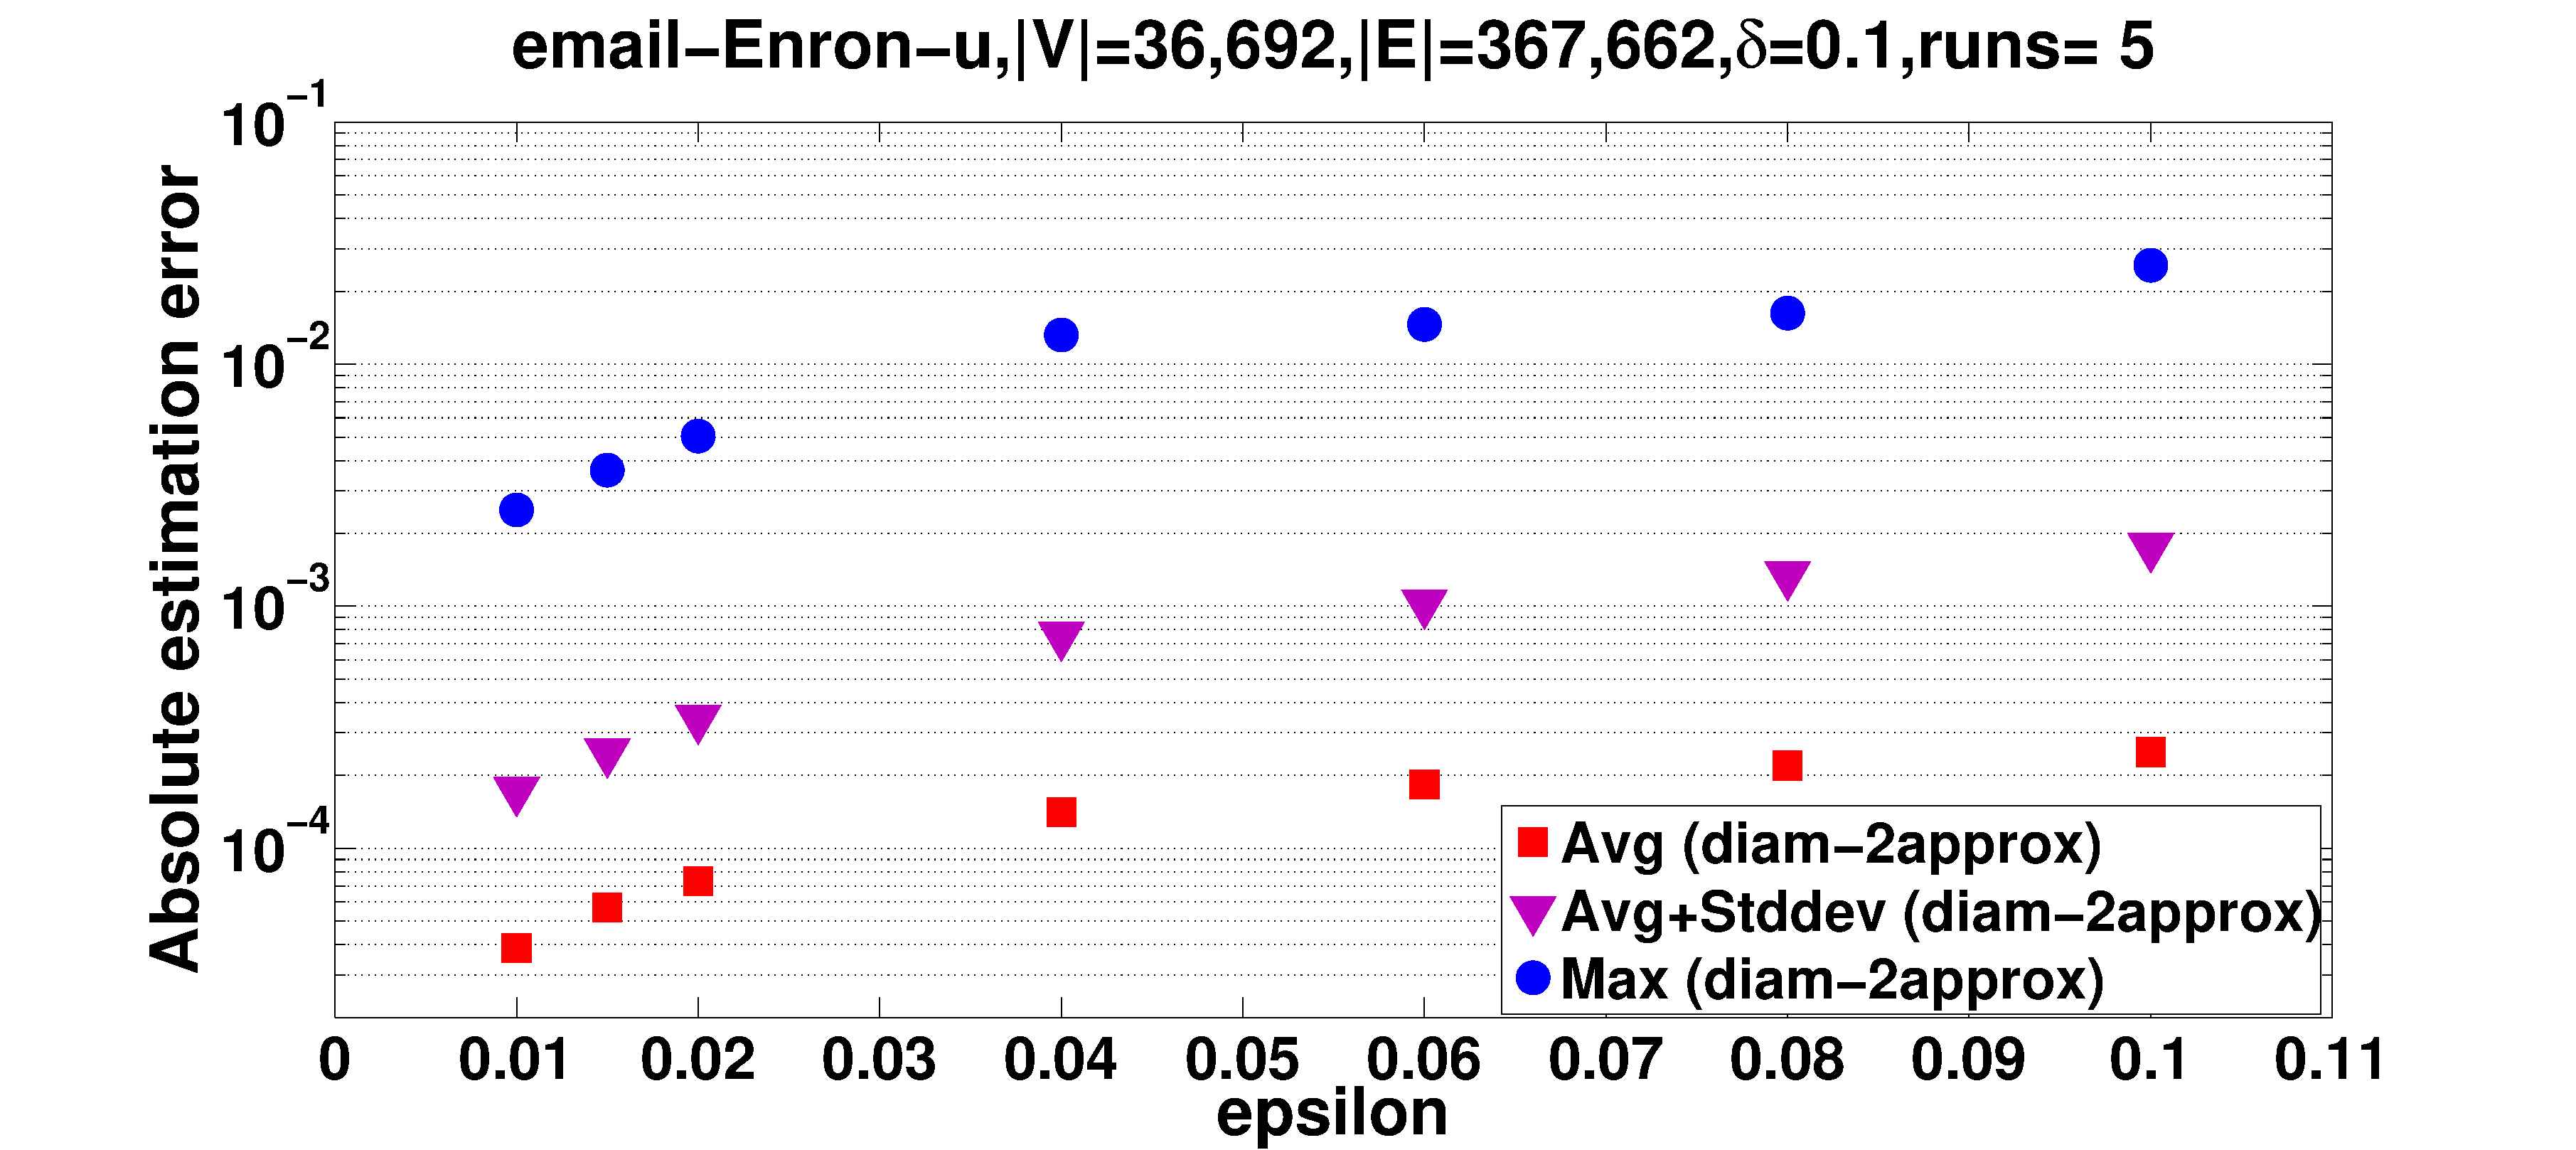
\includegraphics[scale=0.22]{imgs/email-Enron-error.pdf}
  \end{figure}
\end{frame}

\begin{frame}
  \frametitle{How fast is the algorithm?}
  Approximately 8 times faster than the simple sampling algorithm
  \vfill
  Variable speedup w.r.t. exact algorithm (200x -- 4x), depending on
  $\varepsilon$
  \vfill
  \begin{figure}[H]
    \centering
    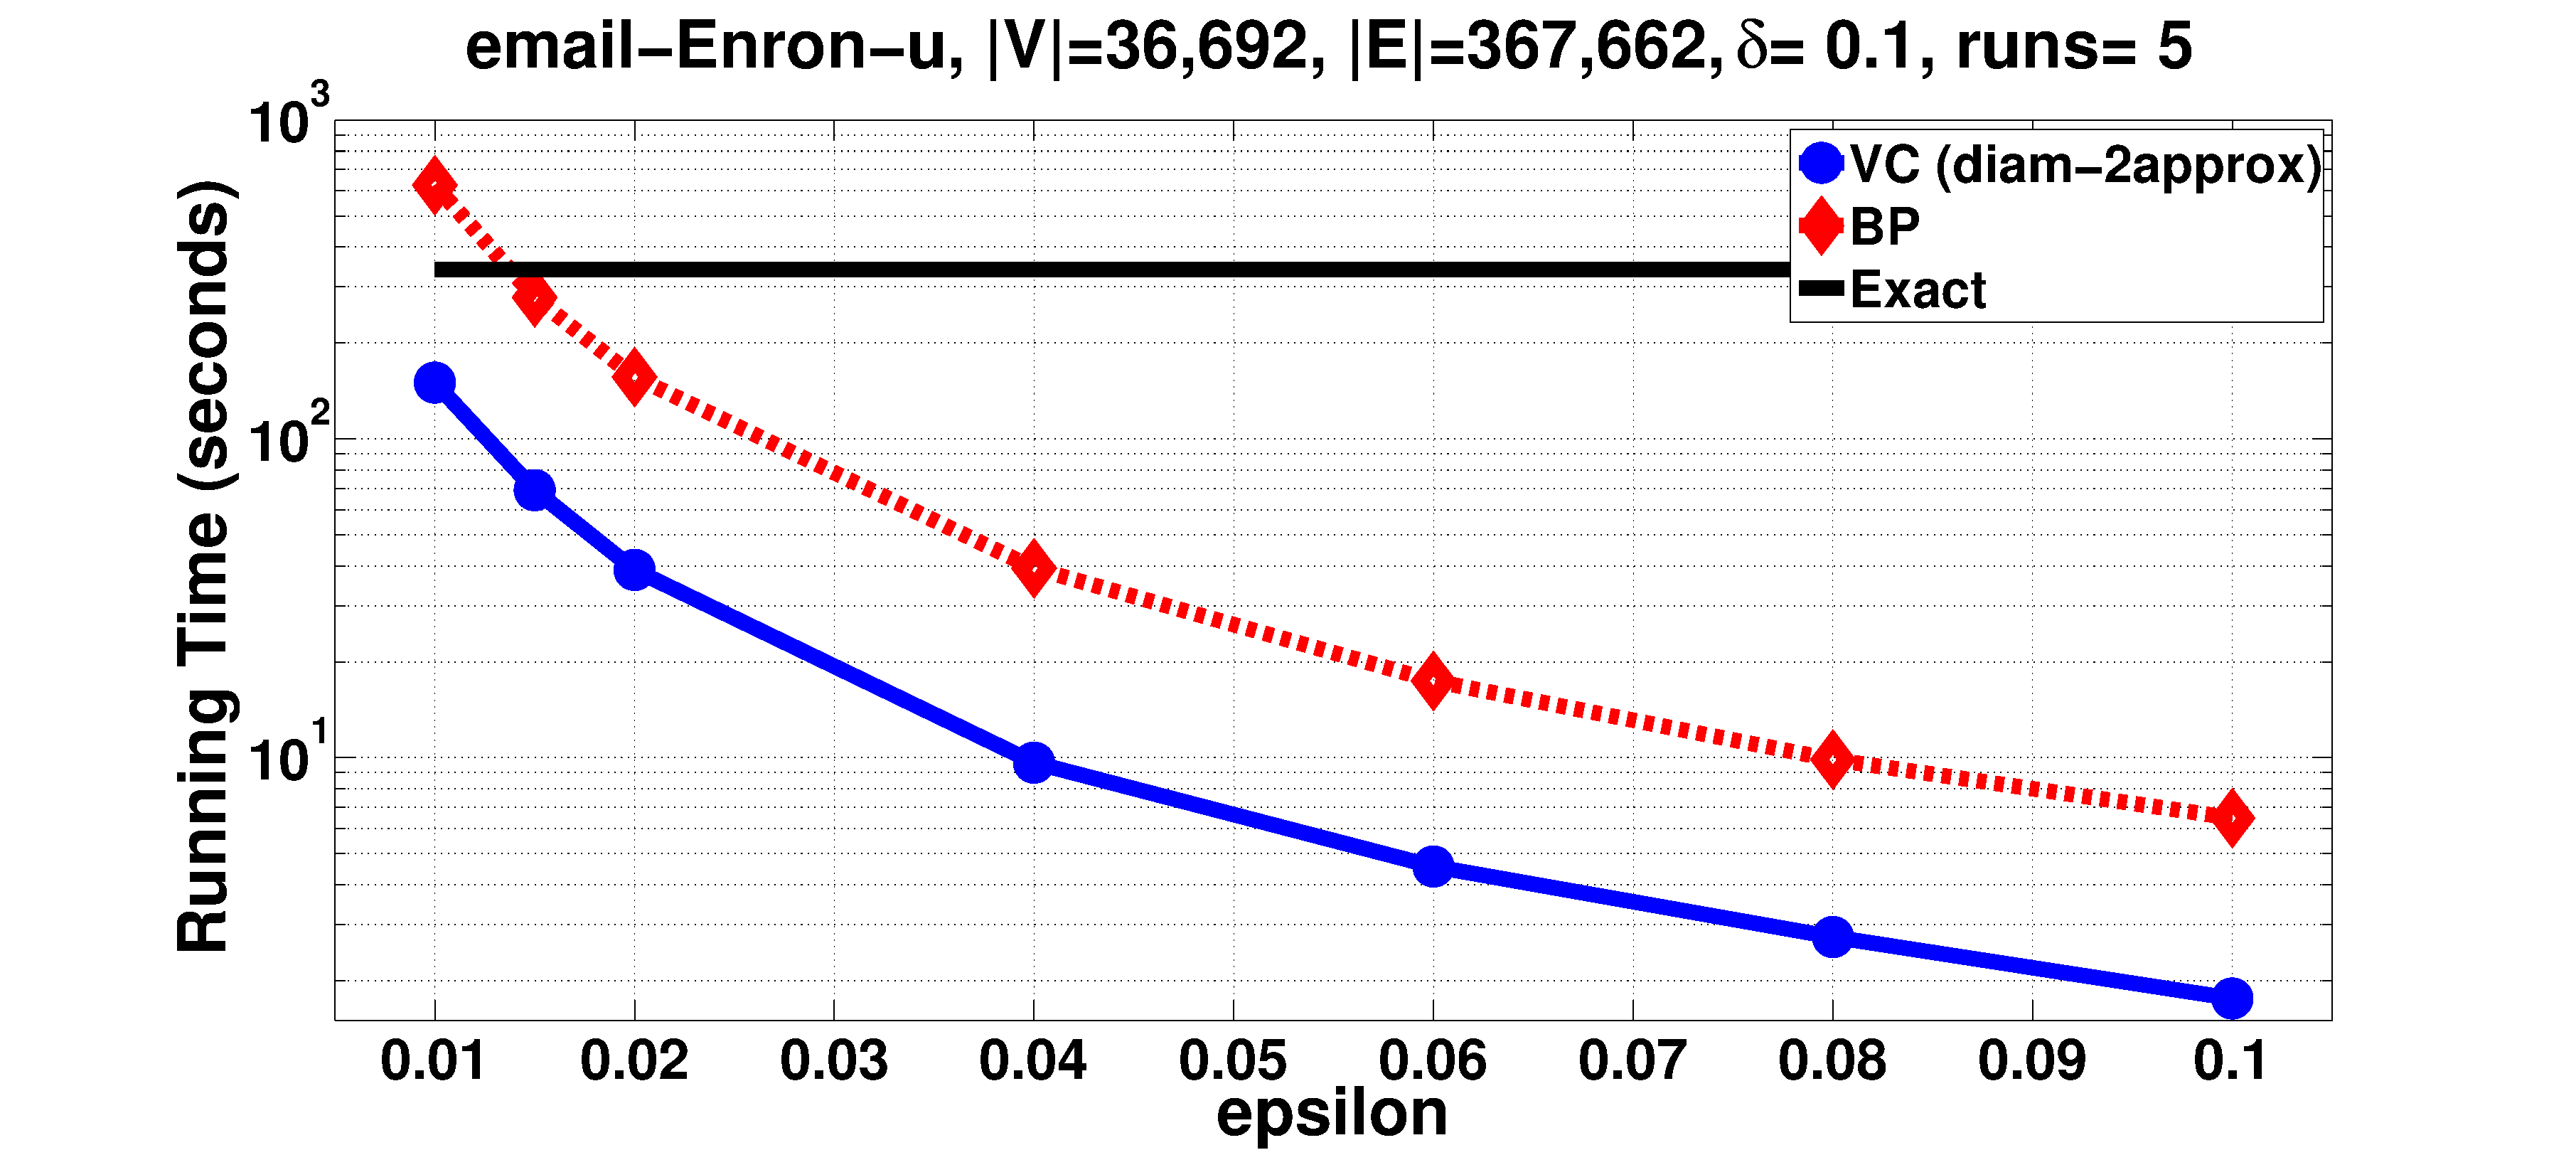
\includegraphics[scale=0.22]{imgs/email-Enron-time.pdf}
  \end{figure}
\end{frame}

\begin{frame}
  \frametitle{How scalable is the algorithm?}
  Much more scalable than the simple sampling algorithm, because the sample
  size does not depend on $n$
  \vfill
  \begin{figure}[H]
    \centering
    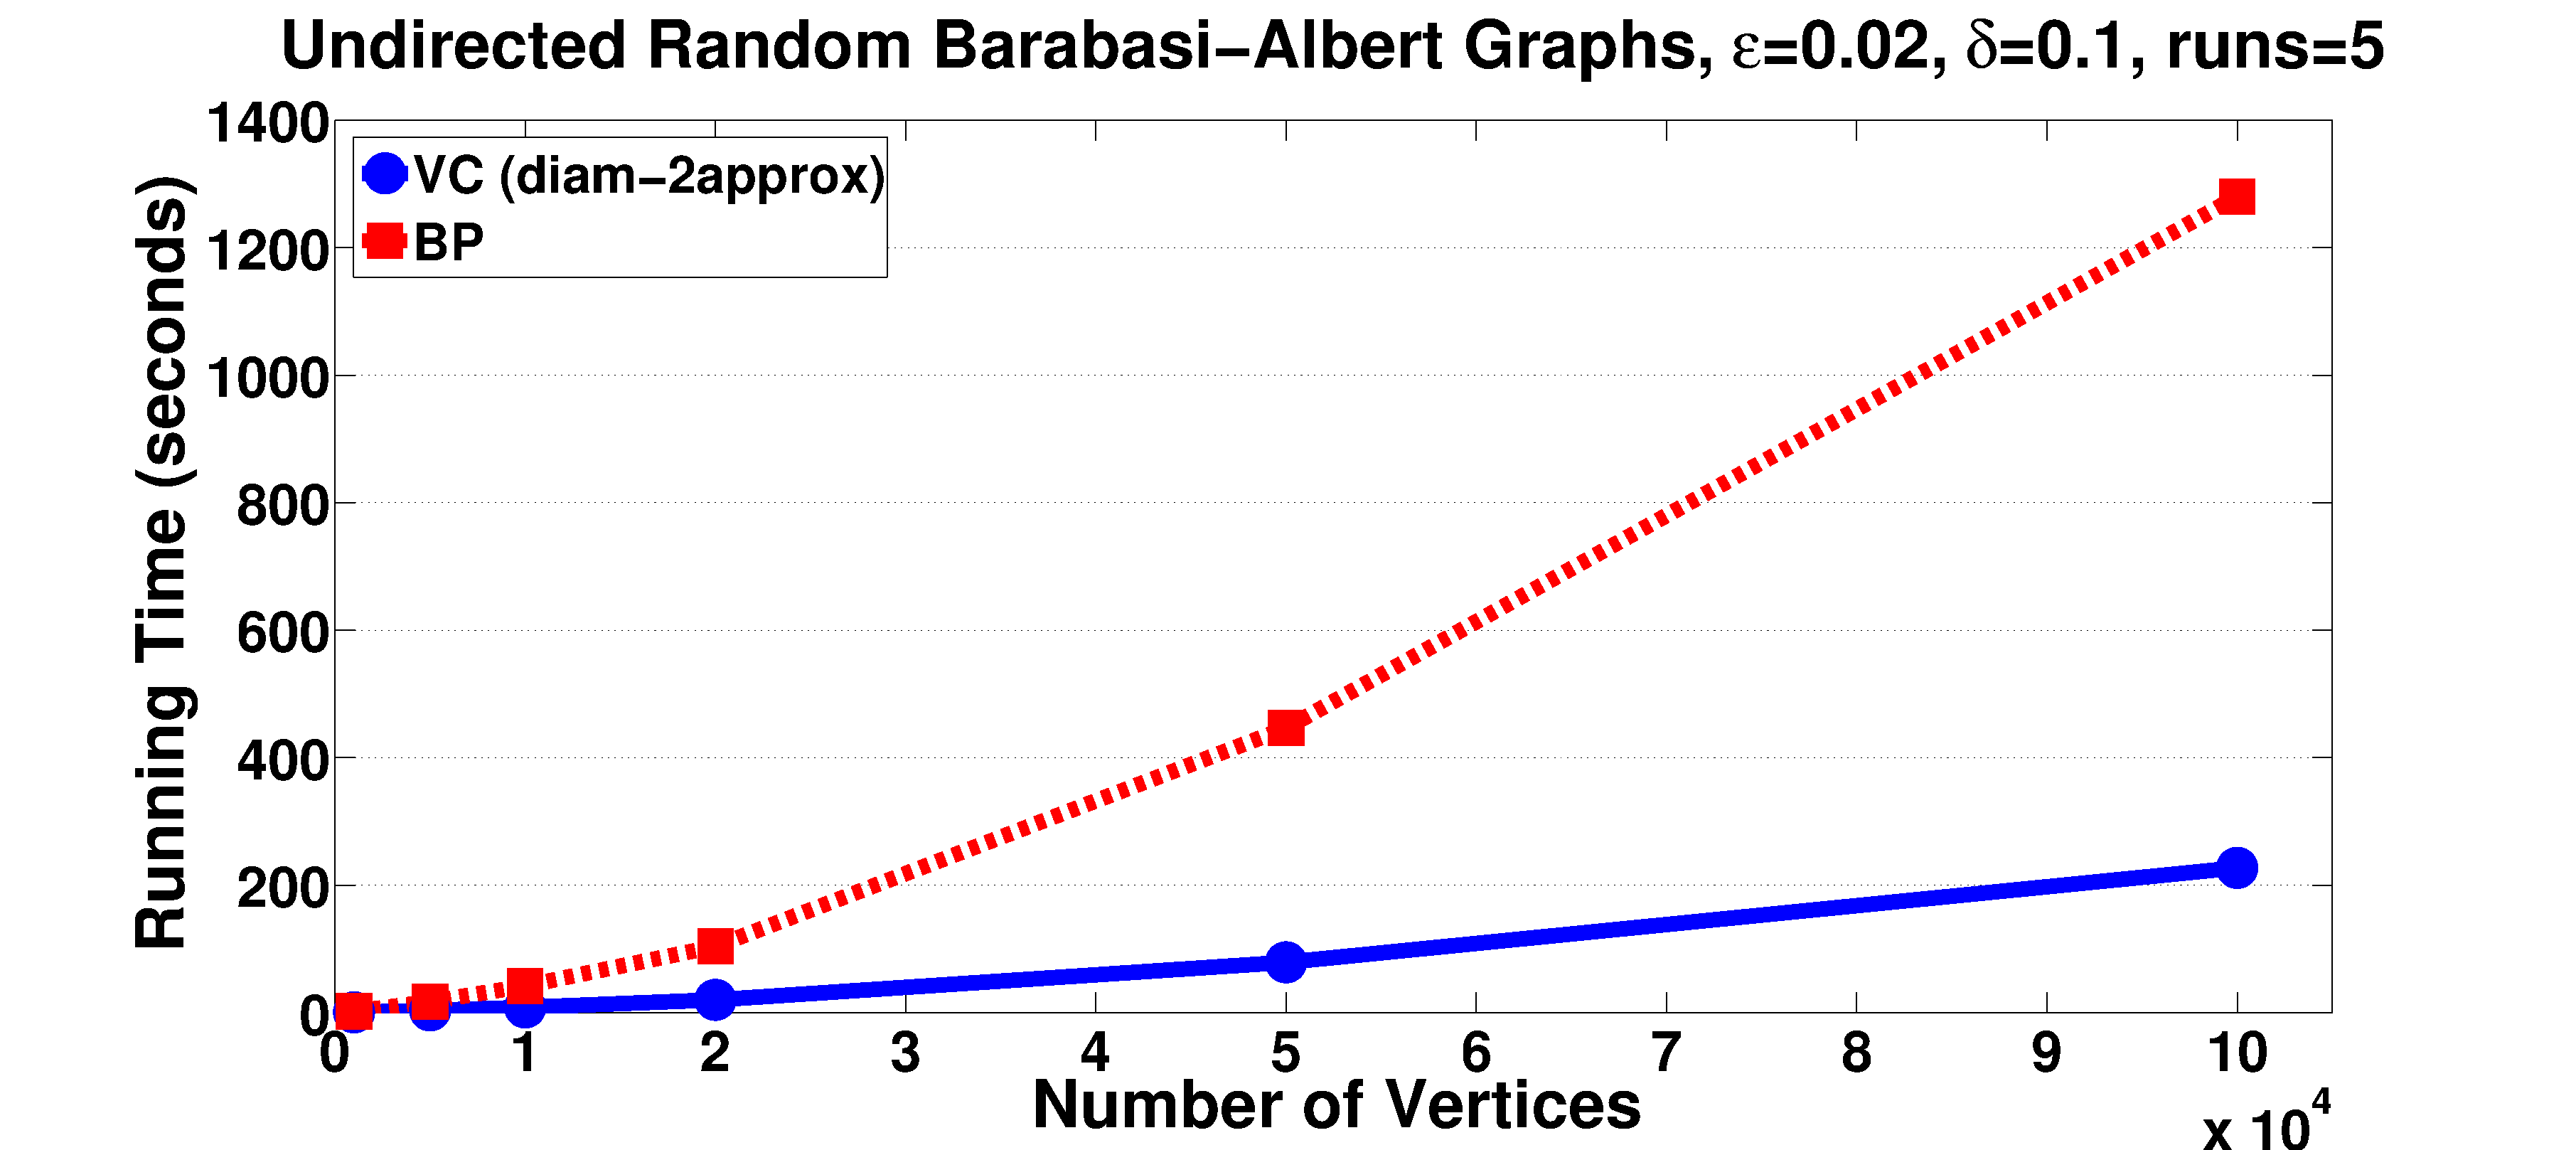
\includegraphics[scale=0.22]{imgs/random-time.pdf}
  \end{figure}
\end{frame}

\begin{frame}
  \frametitle{Conclusions (Betweenness Centrality)}
  \vfill
  We showed a sampling algorithm for betweenness centrality approximation that
  gives probabilistic guarantees on the quality of the approximation for all
  the vertices
  \vfill
  The algorithm samples SPs according to a well-defined distribution, and
  the analysis relies on VC-dimension, which is bounded by the Vertex Diameter,
  a characteristic quantity of the graph that is small in real networks
  \vfill
  The use of VC-dimension makes the algorithm much faster and more scalable
  than previous sampling approaches and than the exact algorithm
\end{frame}

\begin{frame}
  \centering
  \vfill
  {\huge ABRA: Approximating Betweennes Centrality in Static and Dynamic
  Graphs with Rademacher Averages}
  \vfill
  {\large M.~Riondato, E.~Upfal}
  \vfill
  {\large arXiv (2016)}
  \vfill
\end{frame}

\begin{frame}
  \frametitle{What are Rademacher Averages?}
  A measure of complexity of the data analysis task (FIM, in our case)
  w.r.t.~sampling\\
  \quad \inblue{VC-dimension on steroids}
  \vfill
  Definition is \inblue{hairy}: Let $\Sam=\{\tau_1,\dotsc,\tau_{|\Sam|}\}$, the Rademacher
  Average on $\Sam$ is
  \[
    \inblue{\Rade(\Sam)=\expectation_\sigma\left[\sup_{A\subseteq\mathcal{I}}\frac{1}{\ell}\sum_{j=1}^{|\Sam|}
    \sigma_j \phi_A(\tau_j)\left|\right. \Sam\right]}
  \]
  where the $\sigma_i$ are Rademacher rv's and $\phi_A(\tau_i)=\mathds{1}_{\tau_j}(A)$
  \vfill
  The \inblue{important part}: $\Rade(\Sam)$ is a \inblue{sample-dependent
  quantity} and we have:
  \[
    %		\Pr\left(\displaystyle\sup_{A\subseteq\mathcal{I}}|f_\Ds(A)-f_\Sam(A)|\le\inblue{\underbrace{2\Rade(\Sam)
    %			+\displaystyle\sqrt{\frac{2\ln(2/\delta)}{|\Sam|}}}_\eta}\right)\ge 1-\delta
  \]
  We develop a method to \inblue{efficiently compute an upper bound to
  $\Rade(\Sam)$}\\
  \quad So we can compute $\eta$ and \inblue{efficiently check the stopping condition ``$\eta\le\varepsilon/2$?''}
\end{frame}

\begin{frame}
  \frametitle{How can we bound the Rademacher average?}
  We must compute the bound \inblue{efficiently} or we lose the advantages of sampling
  \vfill
  Constraint: We can use \inblue{only} information that can be obtained with a
  \inblue{single scan of $\Sam$}:\\
  \begin{enumerate*}
    \item $\inblue{F_\Sam}$: Frequencies in the sample of the single items ($F_\Sam=\{f_\Sam(a),
      a\in\mathcal{I}\}$)
    \item $\inblue{L_\Sam}$: Lengths of the transactions in $\Sam$ ($L_\Sam=\{|\tau|, \tau\in\Sam\}$)
  \end{enumerate*}
  \vfill
  We use the above and \inblue{a variant of Massart's Lemma} to compute a
  function \inblue{$w$} such that:
  \[
    \inblue{
    \Rade(\Sam)\le \min_{s\in\mathbb{R}^+} w(s,F_\Sam,L_\Sam)
    }
  \]
  The function \inblue{$w$ is convex} so \inblue{we can minimize it efficiently}
  \vfill
  Then we have $\eta= 2 \displaystyle\min_{s\in\mathbb{R}^+} w(s,F_\Sam,L_\Sam) +
  \displaystyle\sqrt{\frac{2\ln(2/\delta)}{|\Sam|}}$ and we stop sampling when
  $\eta\le\varepsilon/2$
\end{frame}

\begin{frame}
  \frametitle{What is the intuition behind $w$?}
  Lemma: $\Rade(\Sam)$ is a function of the frequency distribution of the
  Closed Itemsets in $\Sam$
  \vfill
  The function $w$ is an upper bound to $\Rade(\Sam)$ using information from the sample
  \begin{enumerate}
    \item We use the lengths of the transaction in the sample to understand
      how many CIs there are for each possible frequency
    \item We use the frequencies of the items to bound the frequencies of
      the CIs (anti-monotonicity)
  \end{enumerate}
  This does not require us to compute the CIs from $\Sam$ (they are only for the
  analysis)
  \vfill
  \pause
  By the way, here's $w$:
  \[
    \inblue{
    w(s) =
    \frac{1}{s}\ln\displaystyle\sum_{a\in\mathcal{I}_\Sam}\left(\left(1+\displaystyle\sum_{r=1}^{\chi_a}\displaystyle\sum_{j=1}^{g_{a,r}}2^{\min\{r,h_{a,r}-j\}}\right)e^{\frac{s^2f_\Sam(a)}{2n}}\right)
    }
  \]
  See the paper for details :-)
\end{frame}

\begin{frame}
  \frametitle{How to choose the next sample size ?}
  Prev.~works used a fixed sample schedule increasing according to a user-specified parameter\\
  \quad We can \inblue{compute the next sample size on the fly}: one fewer parameter!
  \vfill
  \inblue{First iteration}: Use a sample $\Sam$ of size at least
  \inblue{$|\Sam|\ge8\displaystyle\frac{\ln(2/\delta)}{\varepsilon^2}$}\\
  \quad Why? It is \inblue{impossible that $\eta\le\varepsilon/2$ at
  smaller sample sizes}
  \vfill
  \inblue{Successive iterations}: multiply the sample size from the previous
  iteration by $\displaystyle\left(\frac{2\eta}{\varepsilon}\right)^2$\\
  \inblue{Intuition:} If the \inblue{frequencies of the items} in the current iteration
  and the \inblue{distribution of the transaction lengths} are the \inblue{same as in the previous
  iteration}, then the stopping condition will be satisfied at this iteration
\end{frame}


\begin{frame}
  \frametitle{Issue with previous approach}
\end{frame}

\begin{frame}
  \frametitle{Rademacher averages}
\end{frame}

\subsection{Approximation Algorithms for Dynamic Graphs}

\begin{frame}
  \centering
  \vfill
  {\huge Fully-Dynamic Approximation of Betweenness Centrality}
  \vfill
  {\Large E.~Bergamini, H.~Meyerhenke}
  \vfill
  {\large ESA: European Symposium on Algorithms (2015)}
  \vfill
\end{frame}

\begin{frame}
  \frametitle{Saving all the DAGS}
\end{frame}

\begin{frame}
  \frametitle{Recomputing the vertex diameter}
\end{frame}

\begin{frame}
  \centering
  \vfill
  {\huge Fully Dynamic Betweenness Centrality Maintenance on Massive
  Networks}
  \vfill
  {\Large T.~Hayashi, T.~Akiba, Y.~Yoshida}
  \vfill
  {\large VLDB: Very Large Databases (2016)}
  \vfill
\end{frame}

\begin{frame}
  \frametitle{A new data structure}
\end{frame}

\begin{frame}
  \frametitle{Conclusions on approximation algorithms}
\end{frame}
